\section{Fundamental objectives for foldings} \label{sec:objectives}

\subsection{Dihedral angles and Mountain/Valley assignments} \label{sec:rulings}

\subsection{Controlling rulings} \label{sec:rulings}

\subsubsection{Local rulings along a DOG} \label{sec:dog_rulings}
\subsubsection{Rulings along a crease} \label{sec:rulings_crease}
If the ruling angles of both surfaces along the crease are $\beta_1(t),\beta_2(t)$, measured by their angles with the tangents, then they satisfy the following \cite{more_on_paper,duncan_folded}:

\begin{equation}
\cot\beta_1(t) = \frac{\alpha'(t)-\tau(t)}{k(t)\sin(\alpha(t))},\cot\beta_2(t) = \frac{-\alpha'(t)-\tau(t)}{k(t)\sin(\alpha(t))}
\end{equation}
Which from here we can deduce (\cite{mathematical_omnibus,duncan_folded}):
\begin{equation} \label{cot_eq}
\begin{split}
\cot\beta_1(t) + \cot\beta_2(t) = \frac{-2\tau(t)}{k(t)\sin(\alpha(t))},\\
\cot\beta_1(t) - \cot\beta_2(t) = \frac{2\alpha'(t)}{k(t)\sin(\alpha(t))},
\end{split}	
\end{equation}
The authors of (\cite{mathematical_omnibus,duncan_folded}) identified two special cases, corresponding to when the above equations vanish. The first correspond to a planar curved fold, i.e. $\cot\beta_1(t) + \cot\beta_2(t) = \tau = 0$ which implies $\beta_1+\beta_2 = \pi$, meaning the rulings are continuation of each other on the flattened surface. In that case the two surfaces are just reflections of each other through the unique osculating plane of the curve (which doesn't change as $\tau = 0$). The second case corresponds to constant dihedral angle along the curve, i.e. $\cot\beta_1(t) - \cot\beta_2(t) = \alpha(t)' = 0$ which implies $\beta_1 = \beta_2$. These two cases coincide in the case $\beta_1 = \beta_2 = \frac{\pi}{2}$ (see \figref{fig:curved_different_rullings}).


\begin{figure} [h]
	\centering
	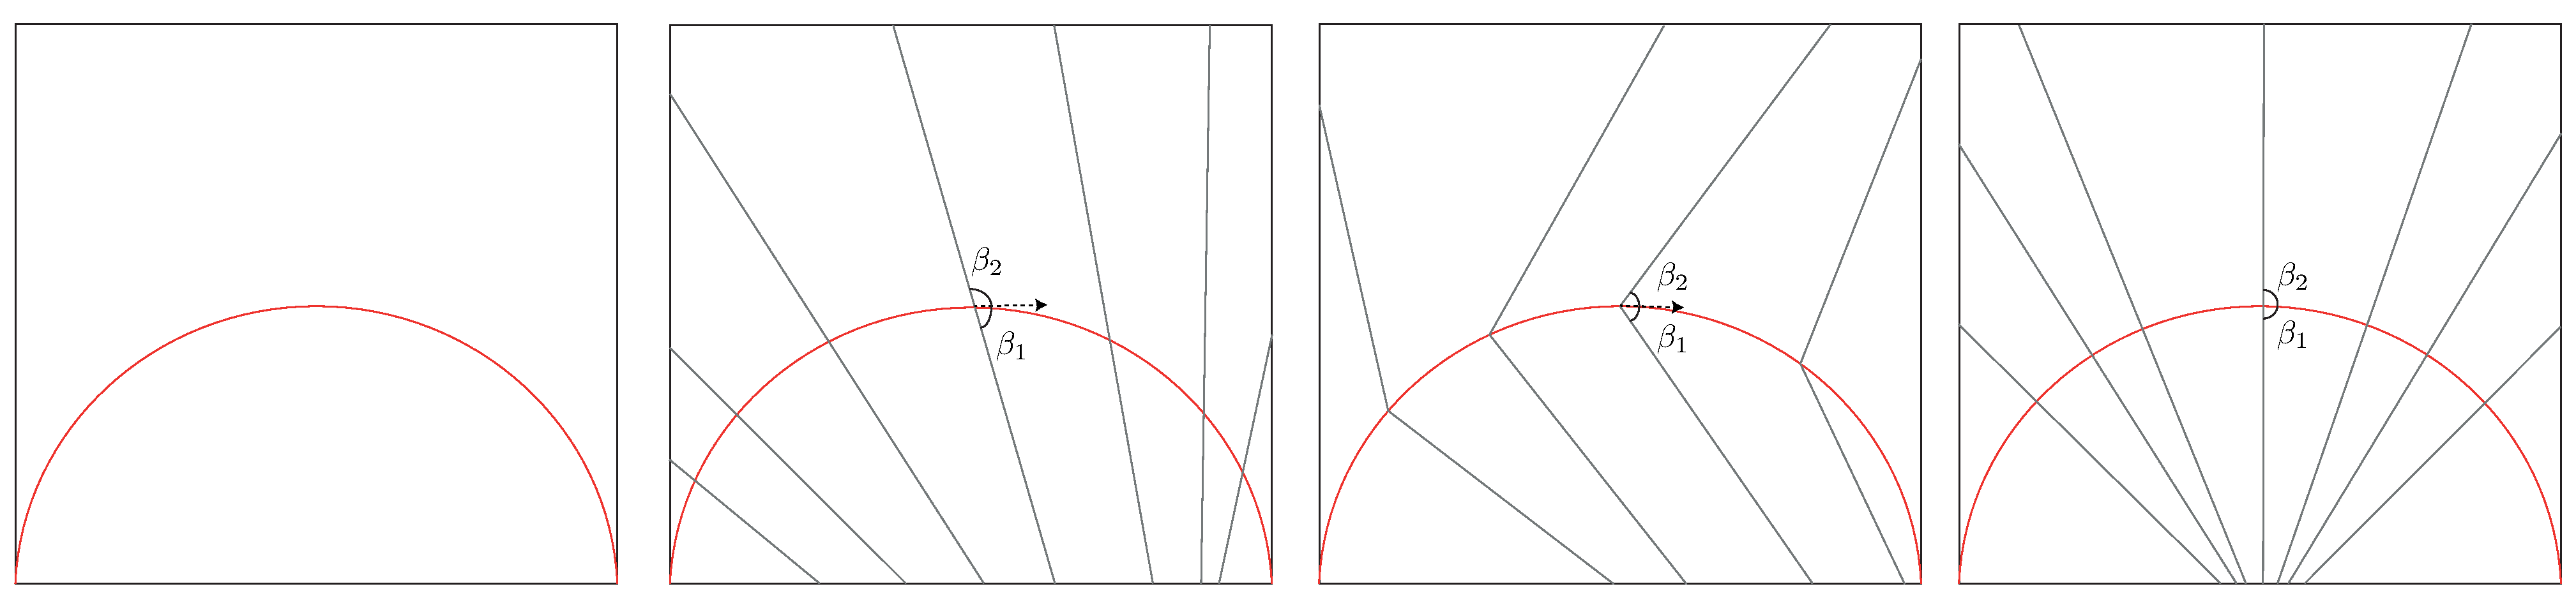
\includegraphics[width=\linewidth]{figures/curved_different_rullings}
	\caption{Different rulings patterns on a circular curved fold, displayed on the flattened configuration. From left to right: A circular curved fold pattern, a ruling pattern corresponding to $\beta_1(t)+\beta_2(t)=\pi$ (implying the curved fold is planar in 3D), a ruling pattern corresponding to $\beta_1(t)=\beta_2(t)$ (implying the dihedral angle between the tangent planes along the curve is constant) and a ruling pattern corresponding to both when $\beta_1(t)=\beta_2(t)=\frac{\pi}{2}$}
	\label{fig:curved_different_rullings}
\end{figure}

\subsection{Rulings objectives on DOG vertices}
